\section{Results and Discussion} \label{sec:results_discussion}
This section presents the results of the security analysis and performance measurements, followed by a discussion of the findings.

\subsection{Security Analysis Results}
The effectiveness of VxLang virtualization was evaluated through static and dynamic analysis attempts to understand and bypass the authentication logic in the case study applications.

\subsubsection{Static Analysis (Ghidra)}
\begin{itemize}
    \item \textbf{Non-Virtualized Binaries:} Analysis was straightforward. Relevant strings (e.g., "Authentication Failed", hardcoded "seno", "rahman") were easily located in the `.rdata` or `.text` sections. Cross-references led directly to the authentication functions. Disassembly clearly showed standard comparison instructions (\texttt{memcmp}, \texttt{strcmp}, or C++ string comparison operators) followed by conditional jumps (\texttt{JNZ}, \texttt{JE}) controlling the flow based on the comparison result (See example Listing \ref{lst:asm_static_nonvirt_snippet} and context in Appendix Listing \ref{lst:asm_static_nonvirt_full}). For cloud variants, the call to the request function and the subsequent check on its return value were identifiable (Listing \ref{lst:asm_static_cloud_snippet}, Appendix \ref{lst:asm_static_cloud_full}). Static patching of the conditional jump instruction to force the "authorized" path was trivial in all non-virtualized cases.
    \item \textbf{Virtualized Binaries:} Static analysis proved significantly more challenging.
        \begin{itemize}
            \item \textit{Instruction Recognition Failure:} Ghidra consistently failed to recognize standard x86-64 instructions within the virtualized sections, reporting large blocks of unknown opcodes or '???' entries. Analysis summaries showed a drastic reduction (often to zero) in the count of recognized instructions and functions compared to the originals (e.g., Fig. \ref{fig:ghidra_summary_qt} vs. Fig. \ref{fig:ghidra_summary_qt_vm} from the thesis).
            \item \textit{Data Obfuscation:} Critical strings like "Authentication Failed" or hardcoded credentials were no longer present as plain text in the binary, preventing simple string searches from locating the relevant code sections. Symbol information was also heavily stripped.
            \item \textit{Control Flow Obscurity:} The clear structure of conditional checks and jumps seen in the original code was replaced by opaque sequences of seemingly unrelated or unknown instructions, making it impossible to identify the core authentication logic or the specific conditional jump to patch statically. The control flow graph became fragmented and uninformative within the virtualized regions.
        \end{itemize}
    Static bypass attempts were unsuccessful due to the inability to locate and understand the relevant control flow logic.
\end{itemize}

% --- Include Ghidra Summary Figures Here ---
% [TODO: Add Figure from Thesis Bab 5: fig:ghidra_summary_qt, relabel as Fig. 1 in journal]
\begin{figure}[!t] % Use !t for top placement preference in IEEE style
    \centering
    % \includegraphics[width=0.9\linewidth]{path/to/ghidra_summary_qt.jpeg} 
    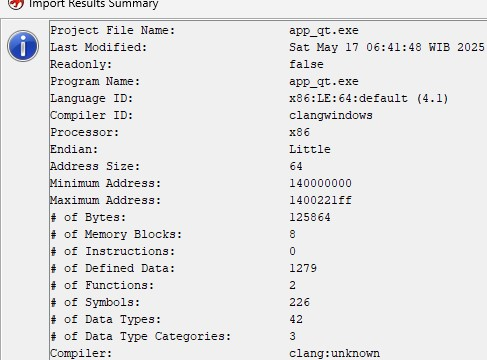
\includegraphics[width=0.9\linewidth]{../assets/pics/app_qt_summary_result.jpeg} % Corrected Path
    \caption{Ghidra Analysis Summary for \texttt{app\_qt.exe} (Non-Virtualized).}
    \label{fig:ghidra_summary_qt} % Referensi baru
\end{figure}

% [TODO: Add Figure from Thesis Bab 5: fig:ghidra_summary_qt_vm, relabel as Fig. 2 in journal]
\begin{figure}[!t]
    \centering
    % \includegraphics[width=0.9\linewidth]{path/to/ghidra_summary_qt_vm.jpeg}
    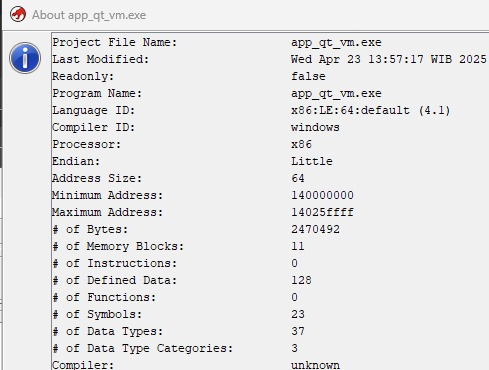
\includegraphics[width=0.9\linewidth]{../assets/pics/app_qt_vm_summary_result.jpeg} % Corrected Path
    \caption{Ghidra Analysis Summary for \texttt{app\_qt\_vm.exe} (Virtualized).}
    \label{fig:ghidra_summary_qt_vm} % Referensi baru
\end{figure}


\subsubsection{Dynamic Analysis (x64dbg)}
\begin{itemize}
    \item \textbf{Non-Virtualized Binaries:} Dynamic analysis corroborated static findings. Setting breakpoints based on string references or near conditional jumps identified statically was effective. Stepping through the code clearly showed the comparison logic and the conditional jump execution. Runtime patching of the jump instruction in x64dbg successfully bypassed authentication (See example Listing \ref{lst:asm_dynamic_nonvirt_snippet} and context in Appendix Listing \ref{lst:asm_dynamic_nonvirt_full}).
    \item \textbf{Virtualized Binaries:} Dynamic analysis faced significant hurdles.
        \begin{itemize}
            \item \textit{String Searching Failure:} Searching for relevant strings in memory during runtime often failed, similar to static analysis.
            \item \textit{Execution Flow Tracking Difficulty:} Stepping through the virtualized code sections was extremely difficult. The instruction pointer (RIP) often appeared to loop within small blocks or jump to seemingly random locations, consistent with execution being handled by the VM interpreter rather than direct native execution (See Listings \ref{lst:asm_dynamic_io_nonvirt_snippet} vs. \ref{lst:asm_dynamic_io_virt_snippet}, Appendix \ref{lst:asm_dynamic_io_comparison_full}). Standard debugging techniques like setting breakpoints based on expected native instructions became unreliable.
            \item \textit{State Obfuscation:} Understanding the program's state (relevant variable values, comparison results) was hindered because the actual logic was executed within the VM's context, which was not directly visible or interpretable through the debugger's view of native registers and memory.
        \end{itemize}
    Dynamic bypass attempts by patching suspected native jump instructions (if any could be identified near the VM entry/exit) were unsuccessful, as the core logic resided within the VM's execution loop.
\end{itemize}

These results strongly indicate that VxLang's code virtualization effectively hinders both static and dynamic reverse engineering attempts using standard tools and techniques.

\subsubsection{Analysis of Lilith RAT}
Static and dynamic analysis were also performed on the Lilith RAT client (original vs. virtualized). Findings mirrored those from the authentication case studies:
    \begin{itemize}
        \item \textbf{Non-Virtualized:} Analysis was feasible. Strings related to commands and functionality were identifiable. Control flow for network communication and command handling could be traced using Ghidra and x64dbg, allowing potential understanding of its mechanisms (e.g., keylogging, remote execution).
        \item \textbf{Virtualized:} Analysis difficulty increased significantly. Ghidra failed to properly disassemble virtualized sections, showing numerous '???' entries and obscuring the logic. Dynamic tracing in x64dbg was severely hampered by the VM execution, making it hard to follow command processing or data flow.
        \item \textbf{Functional Integrity:} Importantly, functional testing confirmed that the virtualized Lilith client remained fully operational, successfully connecting to the server and executing core RAT commands, despite the code transformation.
    \end{itemize}
This indicates VxLang's virtualization hinders analysis even for complex, potentially malicious software, without necessarily breaking its intended functionality.

\subsection{Performance and Size Overhead Results}

\subsubsection{Execution Time Overhead}
The performance impact was measured using QuickSort and AES benchmarks.

\begin{itemize}
    \item \textbf{QuickSort:} As shown in Table \ref{tab:quick_sort_performance} and Fig. \ref{fig:quick_sort_performance}, virtualization introduced substantial execution time overhead. The overhead increased with data size, ranging from approximately 51,400\% for 100 elements to about 20,860\% for 1,000,000 elements. This indicates a significant constant overhead plus a scaling factor imposed by the VM's interpretation loop for the recursive sorting function.
    % [TODO: Add Table/Figure from Thesis Bab 5: tab:quick_sort_performance, fig:quick_sort_performance. Relabel appropriately]
    \begin{table}[!t] % Use table* for full width if needed
        \centering
        \caption{Quick Sort Execution Time Results (ms)}
        \label{tab:quick_sort_performance}
        \resizebox{\columnwidth}{!}{% Resize table to fit column width
        \begin{tabular}{@{}lrrrr@{}}
        \toprule
        \multirow{2}{*}{\textbf{Array Size}} & \multicolumn{2}{c}{\textbf{Non-Virtualized}} & \multicolumn{2}{c}{\textbf{Virtualized}}\\
        \cmidrule(lr){2-3} \cmidrule(lr){4-5}
        & \textbf{Avg Time} & \textbf{Std Dev} & \textbf{Avg Time} & \textbf{Std Dev}\\
        \midrule
        100         & 0.01   & 0.00   & 5.15      & 0.42 \\
        1,000       & 0.09   & 0.00   & 53.08     & 5.52 \\
        5,000       & 0.61   & 0.09   & 300.64    & 26.13 \\
        10,000      & 1.38   & 0.22   & 585.70    & 79.88 \\
        50,000      & 8.45   & 0.73   & 3,434.32  & 592.92 \\
        100,000     & 17.86  & 1.42   & 6,771.09  & 553.09 \\
        500,000     & 106.16 & 5.61   & 29,698.73 & 3,518.63 \\
        1,000,000   & 216.59 & 9.49   & 45,186.90 & 6,198.38 \\
        \bottomrule
        \end{tabular}
        } % End resizebox
    \end{table}

    \begin{figure}[!t]
        \centering
        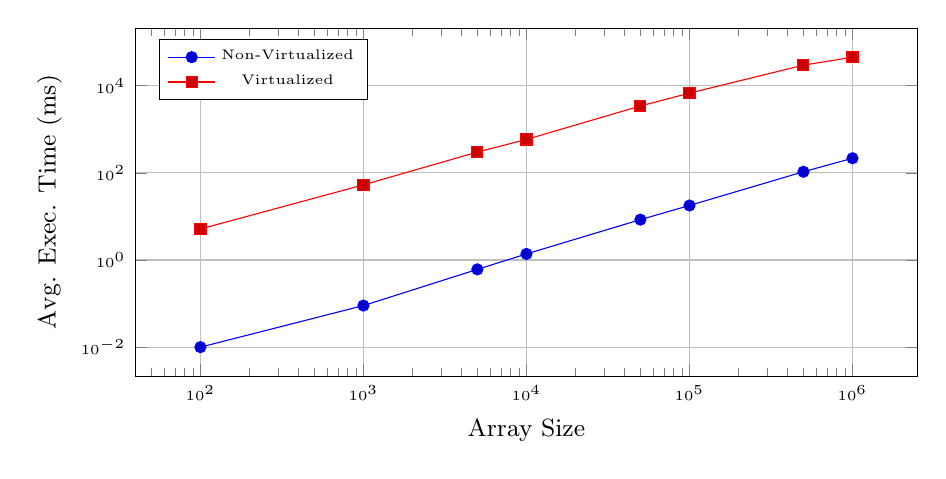
\begin{tikzpicture}
            \begin{axis}[
                width=0.95\columnwidth, % Adjust width to fit column
                height=6cm, % Adjust height as needed
                xlabel={Array Size},
                ylabel={Avg. Exec. Time (ms)},
                xmode=log,
                log basis x={10},
                ymode=log,
                log basis y={10},
                legend pos=north west,
                % title={Quick Sort Performance Comparison}, % Title often omitted in IEEE figures
                grid=major,
                tick label style={font=\tiny}, % Smaller font for ticks
                label style={font=\small},
                legend style={font=\tiny} % Smaller font for legend
            ]
            \addplot coordinates {
                (100, 0.01)
                (1000, 0.09)
                (5000, 0.61)
                (10000, 1.38)
                (50000, 8.45)
                (100000, 17.86)
                (500000, 106.16)
                (1000000, 216.59)
            };
            \addlegendentry{Non-Virtualized};

            \addplot coordinates {
                (100, 5.15)
                (1000, 53.08)
                (5000, 300.64)
                (10000, 585.70)
                (50000, 3434.32)
                (100000, 6771.09)
                (500000, 29698.73)
                (1000000, 45186.90)
            };
            \addlegendentry{Virtualized};
            \end{axis}
        \end{tikzpicture}
        \caption{Quick Sort Execution Time Comparison (Log-Log Scale).}
        \label{fig:quick_sort_performance}
    \end{figure}


    \item \textbf{AES Encryption:} Table \ref{tab:aes_performance} shows that the total time for encrypting 1GB of data increased by approximately 384\%, and decryption time increased by about 510\%. Consequently, the combined throughput dropped dramatically from 416.92 MB/s to 75.98 MB/s (an 82\% reduction). This confirms a significant overhead for cryptographic operations.
    % [TODO: Add Table from Thesis Bab 5: tab:aes_performance. Relabel appropriately]
    \begin{table}[!t]
      \centering
      \caption{AES-256-CBC Performance Results (1GB Data)}
      \label{tab:aes_performance}
        \resizebox{\columnwidth}{!}{%
        \begin{tabular}{@{}lrr@{}}
            \toprule
            \textbf{Metric}                       & \textbf{Non-Virtualized} & \textbf{Virtualized} \\
            \midrule
            Total Encryption Time (ms)      & 2,722.96            & 13,193.51          \\
            Total Decryption Time (ms)      & 2,055.01            & 12,529.90          \\
            Avg. Encrypt Time/Block (ms)    & 0.00272            & 0.01319           \\
            Avg. Decrypt Time/Block (ms)    & 0.00206            & 0.01253           \\
            Encrypt Throughput (MB/s)       & 358.64             & 74.02             \\
            Decrypt Throughput (MB/s)       & 475.21             & 77.94             \\
            Combined Throughput (MB/s)      & 416.92             & 75.98             \\
            \bottomrule
        \end{tabular}
        } % End resizebox
    \end{table}

\end{itemize}

\subsubsection{File Size Overhead}
Table \ref{tab:file_size} shows a consistent increase in executable file size after virtualization. For smaller programs (console, QuickSort, AES), the size increased by over 15-18 times (from ~100-130 KB to ~1.8-1.9 MB). For larger GUI applications (\texttt{app\_imgui}, \texttt{app\_qt}) and the benchmark with embedded data (\texttt{size}), the relative increase was smaller but still significant (e.g., \texttt{app\_imgui} increased by about 55\%, \texttt{size} by 15\%). This overhead is primarily attributed to the inclusion of the VxLang VM runtime and the bytecode representation of the original code.

% [TODO: Add Table from Thesis Bab 5: tab:file_size. Relabel appropriately]
\begin{table}[!t]
  \centering
  \caption{Executable File Size Comparison (KB)}
  \label{tab:file_size}
    \begin{tabular}{@{}lrr@{}}
        \toprule
        \textbf{Program} & \textbf{Non-Virtualized (KB)} & \textbf{Virtualized (KB)} \\
        \midrule
        quick\_sort      & 119        & 1,951      \\
        encryption       & 131        & 1,834      \\
        size             & 97,802     & 112,716    \\
        console          & 105        & 1,942      \\
        app\_imgui       & 1,773      & 2,753      \\
        app\_qt          & 145        & 1,954      \\
        \bottomrule
    \end{tabular}
\end{table}

\subsection{VirusTotal Detection Analysis}
To assess the impact of VxLang virtualization on automated malware detection, both the original and virtualized Lilith RAT client executables were submitted to VirusTotal, a service aggregating results from numerous antivirus engines.

\begin{itemize}
    \item \textbf{Non-Virtualized Lilith:} Detected by \textbf{22 out of 72} engines. Analysis revealed specific threat labels like "trojan.lilithrat/keylogger" and family labels including "lilithrat" and "keylogger". Detections often included specific names like "Backdoor:Win64/LilithRat.GA!MTB" or "Trojan[Backdoor]/Win64.LilithRAT", indicating recognition based on known signatures or specific RAT characteristics.
    \item \textbf{Virtualized Lilith:} Detected by \textbf{18 out of 72} engines, showing a decrease in detection rate. The popular threat label became a generic "trojan", and specific family labels disappeared. Detection signatures shifted towards generic malware, heuristic-based flags, AI/ML detections, or packed/protected software warnings (e.g., "Trojan:Win32/Wacatac.C!ml", "Static AI - Suspicious PE", "ML.Attribute.HighConfidence", "RiskWare[Packed]/Win32.VMProtect.a"). Notably, some vendors that flagged the original version (like Avast, based on thesis observation) no longer detected the virtualized version or provided less specific flags.
\end{itemize}
These results suggest that VxLang virtualization effectively obfuscates static signatures used by many traditional antivirus engines, forcing reliance on less specific heuristic or AI-based methods, and potentially evading detection by some vendors altogether. The detection as "Packed/VMProtect" indicates the virtualization layer itself can be flagged as suspicious by some tools, similar to known packers/protectors.

\subsection{Discussion}
The experimental results clearly demonstrate the core trade-off inherent in using VxLang's code virtualization.

\textbf{Security Enhancement and Detection Evasion:} VxLang provides a substantial barrier against common reverse engineering techniques, applicable even to complex software like the Lilith RAT while preserving its functionality. The transformation into interpreted bytecode neutralizes standard static analysis tools (Ghidra) and significantly complicates dynamic analysis (x64dbg). Furthermore, the VirusTotal analysis indicates that this obfuscation extends to automated malware detection; VxLang effectively hinders signature-based detection, reduces overall detection rates, and forces AV engines towards more generic or heuristic approaches. This capability to evade specific detection signatures adds another layer to its protective potential, aligning with the expected benefits of advanced obfuscation \cite{Ore06, Sal18, Rou13}.

\textbf{Performance Cost:} The security and evasion benefits come at a steep price in terms of performance. The interpretation overhead significantly slows down virtualized code, especially for computationally intensive tasks (QuickSort, AES), potentially rendering indiscriminate application impractical due to severe speed degradation.

\textbf{Size Increase:} The considerable increase in file size, mainly due to the embedded VM runtime, is another factor, particularly relevant for smaller applications or distribution constraints.

\textbf{Practical Implications:} VxLang appears potent for protecting highly sensitive code where security and potentially detection evasion are paramount, and the performance impact on those specific segments is acceptable (e.g., anti-tamper, licensing, core IP). The Lilith case shows it can protect complex logic without breaking it. However, the severe performance cost necessitates a strategic, selective application, targeting only critical sections. The VirusTotal results also imply that while detection is hindered, it's not eliminated, especially by heuristic/AI methods or tools flagging the protection layer itself. The choice between hardcoded and cloud-based authentication showed that protecting client-side logic handling the *result* of validation remains crucial, reinforcing the need for techniques like virtualization on critical checks, regardless of where primary authentication occurs.
